\documentclass[10pt, a4paper, twoside]{article}

% Set up the standard margins for the document
% 42.2 left & 15.5 right is same as Forsling, Neymark
% 21.3 top  & 20 bottom is same as Olofsson
\usepackage[left=19.5mm, right=19.5mm, top=21.3mm, bottom=20mm]{geometry}

\usepackage{subcaption}
\usepackage{float}

% Input file character encoding (kinda useless if we don't
% use åäö and stuff, but it doesn't hurt to have it)
\usepackage[utf8]{inputenc}
%\usepackage[swedish]{babel}

% Block Comments
\usepackage{comment}

% No indentation in new paragraph
\usepackage{parskip}

% To include graphics
\usepackage{graphicx}

\usepackage{epstopdf}	% Enable the usage of .eps images

% More mathematical symbols and fonts
\usepackage{amsmath}
\usepackage{amsfonts}
\usepackage{amssymb}

% Simple list
\usepackage[ampersand]{easylist}
\ListProperties(Hide=100, Hang=true, Progressive=5ex, Style*=$\bullet$ ,
Style2*=-- ,Style3*=$\circ$ ,Style4*=\tiny$\blacksquare$ )


% Clickable internal links
\usepackage{hyperref}
\usepackage[all]{hypcap} % without this the link takes you to the caption, not the top of the image
\hypersetup{ % Settings for links in documnet
	setpagesize = false, % Don't allow hyperref to change page size. Tips från Micke Olofsson
	colorlinks = true,   % No boxes around links
	linkcolor = black,citecolor = black,filecolor = black,urlcolor = black, % don't color links
}

% To include to first page pdf file
\usepackage{pdfpages}

% Add section number to equation and figure number (ex: 5.11 instead of simply 11)
\numberwithin{equation}{subsection}
\numberwithin{figure}{section}
\numberwithin{table}{section}

% Show program code listings in document
\usepackage{listings}

%
% Header stuff
%
\usepackage{fancyhdr}
\setlength{\headheight}{15pt}

\fancyhf{}
\fancyhead[LE, RO]{\thepage}
\fancyhead[RE]{TSBK03 2013: Technical Report}
\fancyhead[LO]{Extrapolate and Conquer}

\fancypagestyle{plain}{ %
\fancyhf{} % remove everything
\renewcommand{\headrulewidth}{0pt} % remove lines as well
\renewcommand{\footrulewidth}{0pt}}
%
% End header stuff
%




\begin{document}

% First page

\includepdf{Cover/cover.pdf}


% Project identity page
\newpage
\pagestyle{fancy}
\pagenumbering{roman}
\setcounter{page}{2} % sets the current page number to 2 

\begin{center}
    \vspace*{4\baselineskip}

	\textbf{\huge Extrapolate and Conquer} \\
	\vspace*{0.5\baselineskip}
	Teknik för avancerade datorspel, HT 2013 \\
	Department of Electrical Engineering (ISY), Linköping University
	
	\vspace*{2\baselineskip}
	\textbf{\LARGE Participants}


	{\footnotesize 
	\begin{tabular}{|p{2.7cm}|p{1cm}|p{2cm}|p{3.4cm}|}
		\hline
		\textbf{Name} & \textbf{Tag} & \textbf{Phone} & \textbf{E-mail} \\
		\hline
		Gustav Häger & GH & 070--649\,03\,97 & gusha124@student.liu.se \\
		\hline
		Alexander Sjöholm & AS & 076--225\,11\,74 & alesj050@student.liu.se \\
		\hline
		Mattias Tiger & MT & 073--695\,71\,53 & matti166@student.liu.se \\
		\hline
	\end{tabular}
	}

{\footnotesize 
\vspace{0.5\baselineskip}
\vspace{1\baselineskip}

\textbf{Examiner}: Ingemar Ragnemalm, ingis@isy.liu.se \\
}

\end{center}



% table of contents
\newpage
\tableofcontents
\listoffigures
\listoftables

% Blank page
%\newpage
%\thispagestyle{empty}
%\mbox{}



%
% Content start
%
\newpage
\pagenumbering{arabic}

\newpage
\section{Introduction}
\label{sec:introduction}
The aim of this project was to develop a computer graphics application combining several state-of-the-art techniques into a beautiful world. 
\begin{figure}[H]
  \centering
  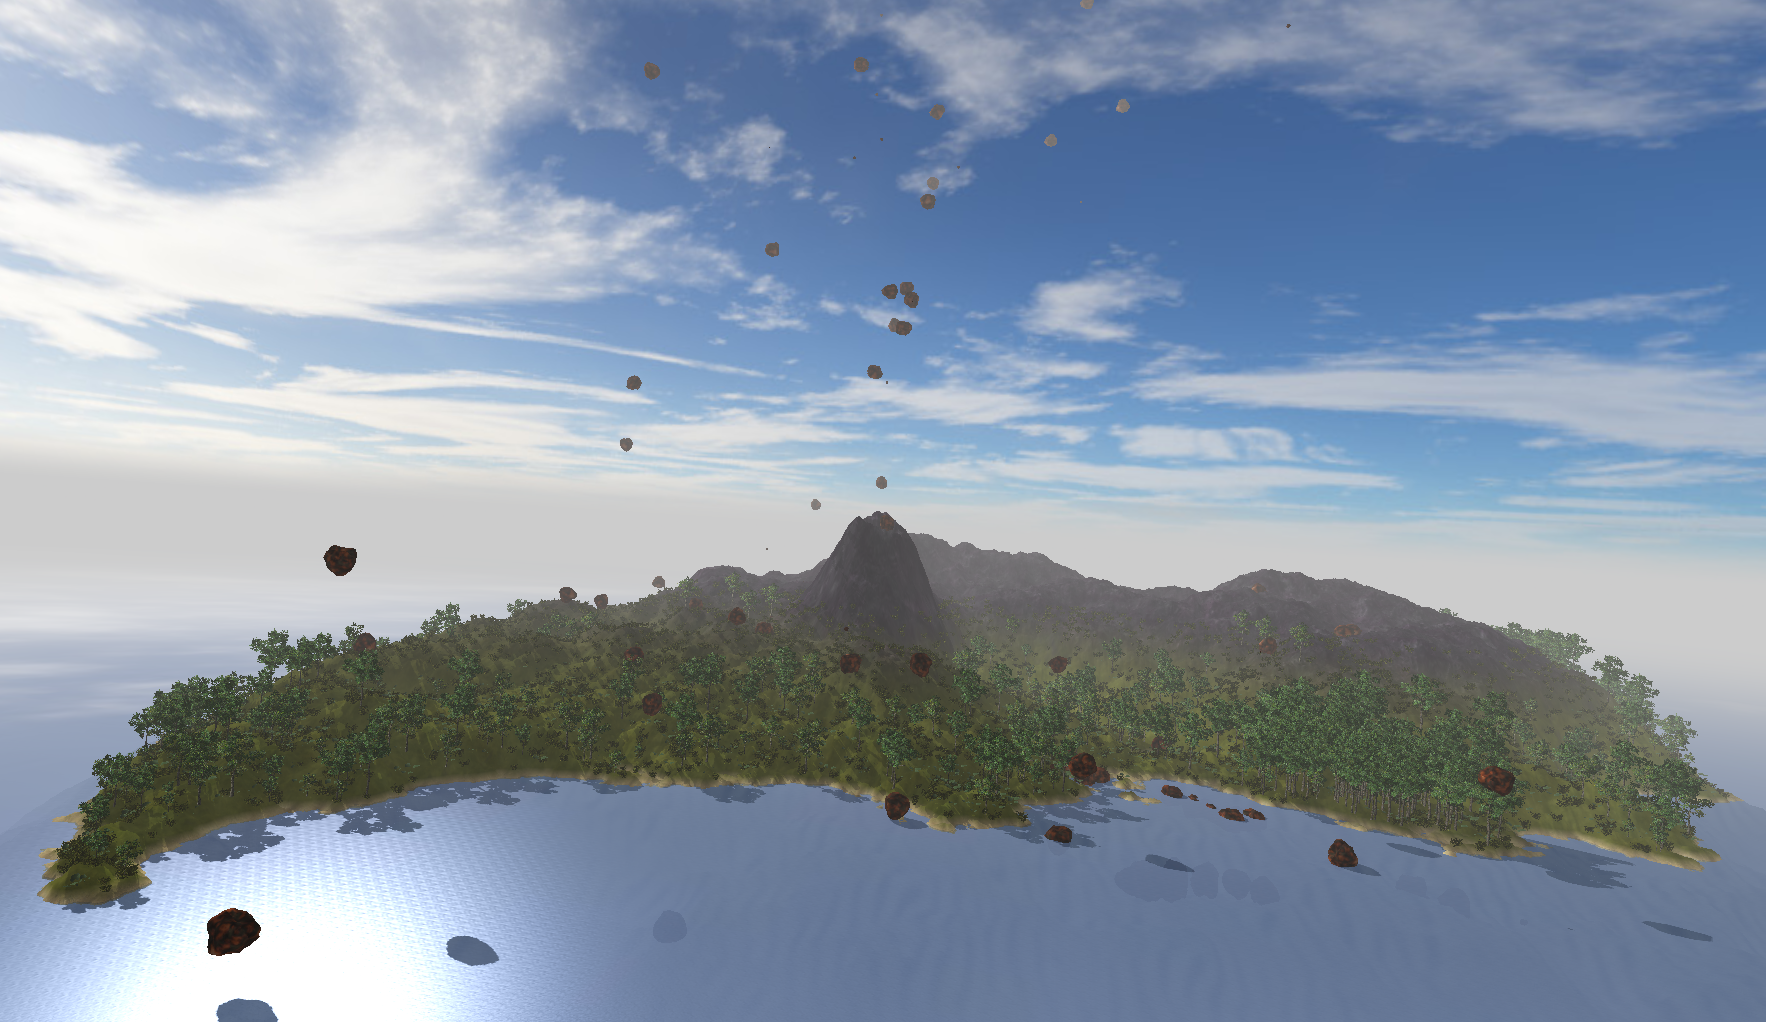
\includegraphics[width=1.0\linewidth]{images/front.png}
  \caption{A beautiful world.}
  \label{fig:beautifulIsland}
\end{figure}%

\newpage
\section{System Core}
\label{sec:Core}
We built and uses an Entity System as an underlying game engine framework.
The idea behind an entity system is that objects should be treated as pure aggregations of data containers, with game logic being separated from objects all together. Instead of having deep class hierarchies and chained method calls, logic for managing specific components is batched on all such components in the system. This provides some advantages over other approaches such that the architecture becomes more flexible and expendable. It is clearer how to add functionality and especially where. Another advantage from the batching is the possibility of much higher performance (maximizing caching and minimizing cache misses) as well as simplifying parallel processing.

\subsection{Entity System}
An Entity System consists of three main parts: Entities, Components and Systems.
An Entity is simply a label or identifier of an object. A Component is a pure data containers, and each entity has a collection of none to several different components. A System consist of logic for working with primarily one, but sometimes several, components. So, an object is an entity label and a collection of components that belong to it. The object is updated by different systems performing tasks on the components. An example used in this project is seen in figure \ref{fig:EntityComponentSystemExample}.
\begin{figure}[H]
  \centering
  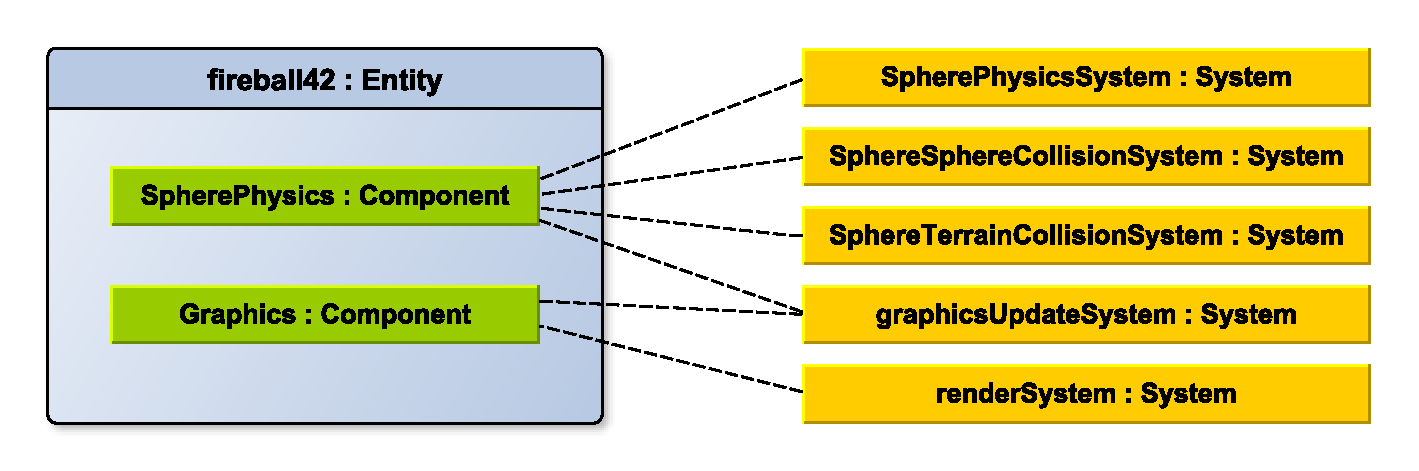
\includegraphics[width=0.9\linewidth]{images/EntityComponentSystemExample.eps}
  \caption{Caption}
  \label{fig:EntityComponentSystemExample}
\end{figure}
(TODO: reformulera och skriv nedan mer flytande och omarbetat)\\
* The idea behind: Systems perform on ALL components of a certain type, which is fetched from the EntityManager.\\
* Our system allows for components to require other components. This means that systems which work on multiple components can be proven to always work by fetching the component which require the others. The require check is performed at compile time and code is generated to handle the specific requirement-tree specified. The program writes part of itself to be maximum efficient and robust, by specifications by the developer in the source code.\\
* Easy to use (a natural work flow of what goes where and how to solve problems. minimal overhead to use the system), easy to maintain, easy to extend, extremely efficient, trivial to parallelize calculations, verifies consistency at compile time...


\begin{lstlisting}
 Entity & entity = entityManager.createEntity();
 
 entity->add<SpherePhysics>();
 entity->add<Graphics>();
 
 SpherePhysics & physics = entity->get<SpherePhysics>();
 physics.position = QVector3D(0.0, 0.5, 1.0);
 physics.friction = 0.5;
 ...
 
 Graphics & graphics = entity->get<Graphics>();
 graphics.object = new Object(resourceManager->getModel("stone1"),
                              resourceManager->getShader("phongTex"),
                              resourceManager->getTexture("lava1")); 
\end{lstlisting}

\begin{lstlisting}
 entity->has<Component>();
 entity->add<Component>();
 entity->remove<Component>();
 entity->get<Component>();
\end{lstlisting}

\begin{lstlisting}
  // If additional Components are required, add these aswell (recursively)
    meta::FOR_EACH< typename Component::REQUIRED_COMPONENTS, // List (items) to iterate over
    
                    ADD_COMPONENT,                           // Template to apply
                                                             // on each item.
                    std::tuple<Component, Components...>,    // Additional template
                                                             // parameters to above template.
                    std::tuple<Entity<Components...>&>       // Argument types to the above
                                                             // templatet's execute-function.
                  >::execute(entity);

\end{lstlisting}

\subsection{Rendering}
The rendering system is outside the entity system mainly because it is the largest part, and it was not known in the start of the project what information it needed exactly, so rather than potentially locking ourselves to an unusable architecture the renderer was placed beside the entity system rather than as a part of it.

The rendering is done in two major passes, the first calculates the shadows and second draws the world using the shadow information calculated in the first pass.

In order to correctly draw the growth some form of transparency was needed as the foilage used partly transparent textured polygons. As the textures where either completely transparent or completely opaque a simple alpha test was sufficient rather than sorting the trees. However the mipmaps calculated by opengl for the foilage where completely broken by the transparency, so these are disabled for the trees.

In order to be able to draw a sufficient number of trees and bushes a simple form of instancing is used. Each type of tree and bush exists in a separate list, that contains the model and texture for that particular object and an array of model matrices to be uploaded to a shader as an array of uniforms.

The rocks on the other hand are drawn individually, using only a reference to a shared model objects, and individual matrices, as well as a specified shading program, thus the rocks could be drawn using individual shaders if it was needed.

The water is always drawn last, as it is the only object in the world that is sempitransparent, this does have the consequence of making the trees invisible from under the water though.

In general this demonstrates the need to for a rendering pipline that does not connect a particular shader to a particular object, but rather connects objects to different shaders, so that the shader program can be selected first, and then all the objects using a particular shader drawn.

Due to a rather lousy bush model with a great deal of z-fighting in itself the depth mask is disabled while drawing bushes, as this is considerably faster than finding and creating new models.

\subsection{Physics}
The physics used in this game is divided into three systems, all three processing all \textit{SpherePhysics} components in the Entity System. The physics is limited to 3D sphere physics as well as the interaction between spheres and a terrain mesh.

\subsubsection{SpherePhysics}
SpherePhysics is a component dedicated to physics data, its content is seen in the code below. The physics is capable of running backwards as well as forwards.
\begin{lstlisting}
 struct SpherePhysics : public Component<> {
    const std::string getName() override { return "SpherePhysics"; }

    float mass;                     // m            (Positive)
    float elasticity;               // epsilon      (Between 0 and 1)
    float friction;                 // friction     (Between 0 and 1)
    float momentOfInertia;          // For a sphere: 6/12*m*radius^2
    float gravitationalConstant;    // g            (Positive. in Sweden at sea level: 9.82)

    QVector3D force;                // F = ... external events ...
    QVector3D linearMomentum;       // P = Integral( F, dt );
    QVector3D velocity;             // v = P / m;
    QVector3D position;             // x = Integral( v, dt );

    QVector3D torque;               // T = ... external events ...
    QVector3D angularMomentum;      // L = Integral( T, dt );
    QVector3D angularVelocity;      // w = L * Inverse(I)
    QQuaternion angularVelocity2;   // w = L * Inverse(I)
    QQuaternion rotation;           // r = Integral( w, dt );

    float radius;                   // Radius of the sphere
    QVector3D collisionVector;      // The sum of the vectors from all collisions

 };
\end{lstlisting}

\subsubsection{SpherePhysicsSystem}
The sphere physics are based on the physics lab, with a generalization to 3D and using quaternions as the representation for rotation. The system require the current time step $dt$. which is used as the integration step in the Euler-forward integration used. This was sufficient for our needs, with no more advanced integration schemes necessary.\\
\\
The spheres are affected by external forces and torques, which then updates the rest of the physical states. At the end, any forces and torques has been handled and are set to zero, and finally the ever present gravitational force is added.

\subsubsection{SphereSphereCollisionSystem}
The sphere-sphere collision handling are based on the physics lab, with a generalization to 3D. The collision is handled by reversed impulse. Collisions give rise to torque, making he collisions seem very realistic.

\subsubsection{SphereTerrainCollisionSystem}
The sphere-sphere collision handling uses the terrains height and normal at the bottom of the sphere. It is otherwise similar to the SpherePshereCollisionSystem apart from that the terrain is considered to have infinite mass. A normal force is applied to the object to minimize noise from the gravity force. A friction force can be used if a more realistic collision is desirable. In our demonstration it isn't used since we had a limited amount of fire balls, so the fewer that got stuck on land the longer the volcano could spew out new fire balls.


\newpage
\section{Graphics}
\label{sec:Graphics}
Graphics graphics.

\subsection{Generating a World}

A world is easily divided into different aspects. There are the sky, the oceans and the land. The land contain different terrain, with different types of ground and vegetation. There is a sun orbiting the world, casting rays of light and in the process creating reflections and indirectly making shadows.\\
\\
A procedural world is generated by carefully chosen algorithms. Our world is procedurally generated anew in a new unique constellation on every run, or a seed can be provided to generate specific worlds. The terrain is first formed, then the ground texturing and the vegetation, both dependent on properties of the terrain. The shadows depend on the sun and the waves on the terrain as well as on time itself.

\subsubsection{Sky}
The sky is achieved using a high-resolution texture of a sky mapped to a skybox. The mathematical location of the sun is placed as close as possible to the sun appearing in this texture. This gives shadows and shading a natural feel. The texture has been manually modified at the horizon to fade towards a shadowish gray color. The color is the same as the one objects are distance-fogged with. This makes the sky melt into the ocean in a very nice way. 

\subsubsection{Ocean}
// TODO  Tiger \\
Normal-mapped square with moving normal map. Makes the water glister/glitter from a far.\\\\
FIGURE(water that glister)
\\
Waves on the beaches is made by having several sinus waves aggregate horizontally to vary the wave fronts, and by having a sinus wave that control the vertical assent/decent of the waves.\\
\\
FIGURE(showing nice waves)
\begin{figure}[H]
\begin{subfigure}{.5\textwidth}
  \centering
  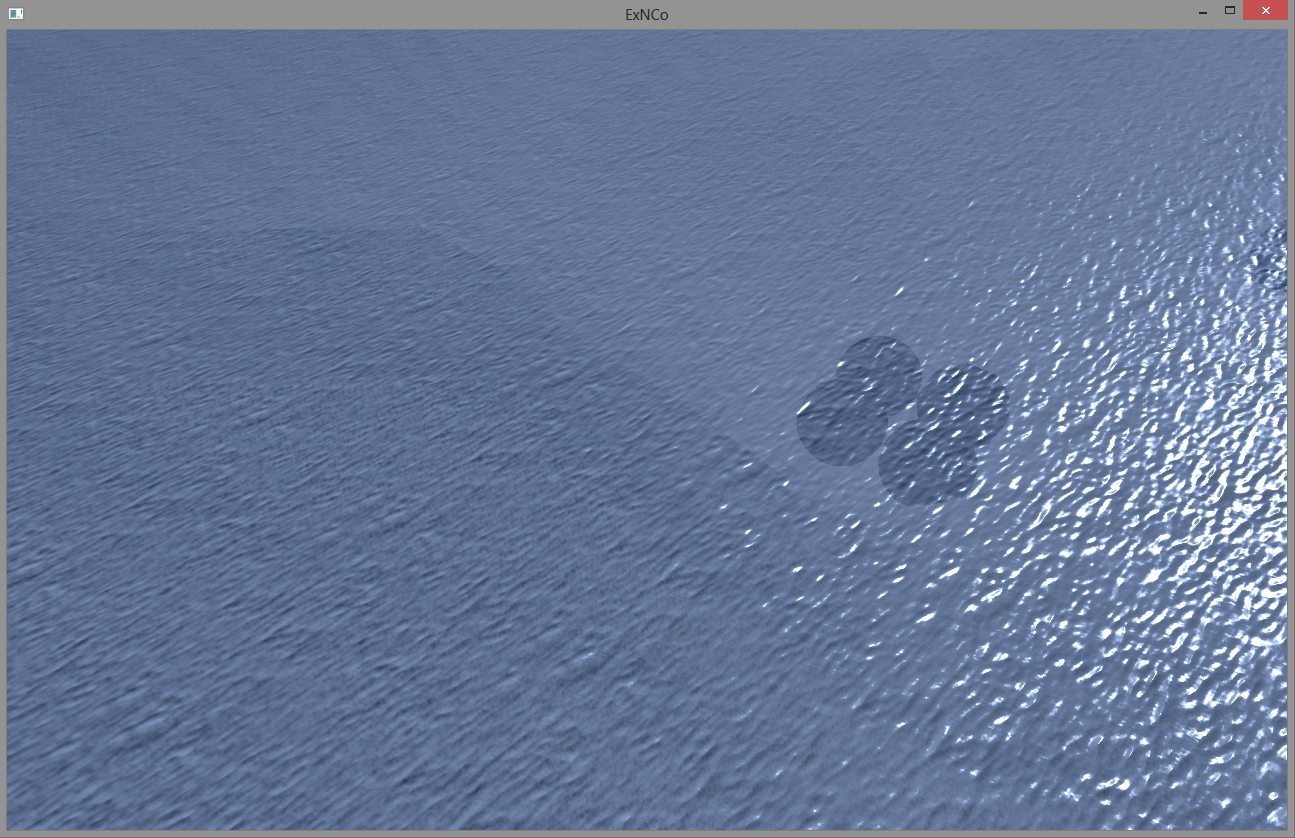
\includegraphics[width=0.9\linewidth]{images/waterWaves.png}
  \caption{Waves.}
  \label{fig:waterWaves}
\end{subfigure}%
\begin{subfigure}{.5\textwidth}
  \centering
  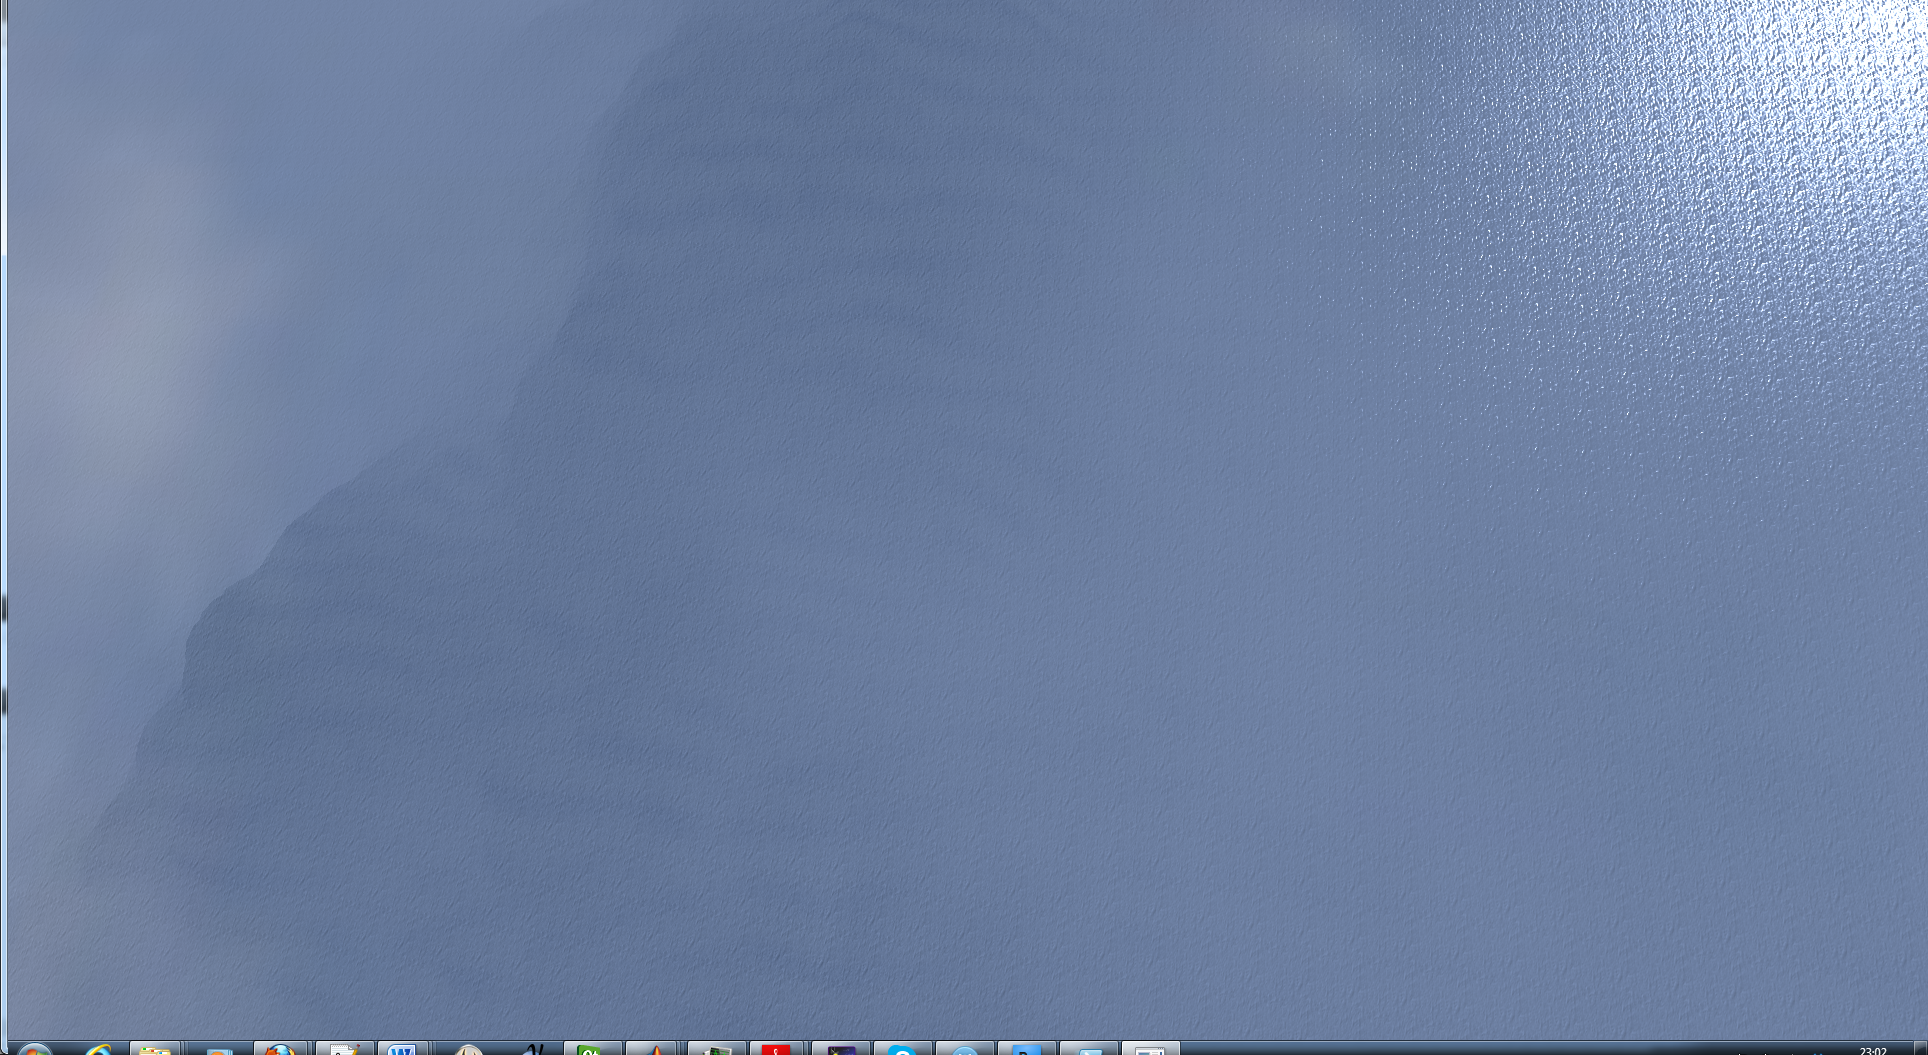
\includegraphics[width=0.9\linewidth]{images/waterGlimmer.png}
  \caption{Glistering water.}
  \label{fig:waterGlistering}
\end{subfigure}
\caption[Noise comparison]{\textit{Comparison of noise functions}}
\label{fig:water}
\end{figure}

\newpage
\subsubsection{Terrain}
The terrain is generated by sampling a noise function and translating its value into a height for the current vertex. The noise in this case originates from a Simplex function. However, to get a realistically looking terrain one it is not sufficient to sample this function only once for every vertex.

Fractional Brownian Motion is calculated by sampling the Simplex function at different frequencies and calculating a weighted sum over the samples \cite{FracBrownMotion}.  The result is a nice looking height map. 

\begin{figure}[H]
\begin{subfigure}{.5\textwidth}
  \centering
  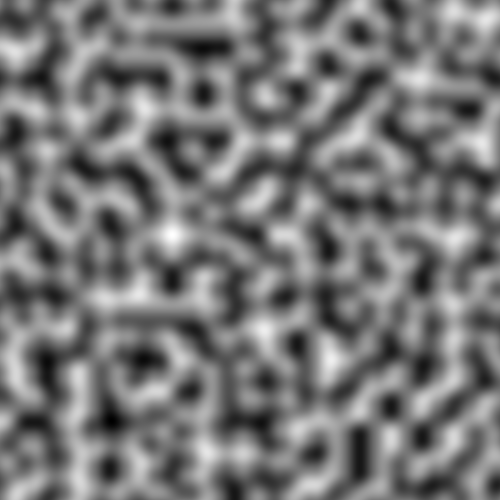
\includegraphics[width=0.9\linewidth]{images/Simplex.png}
  \caption{Height map generated from single-octave simplex noise}
  \label{fig:sub1}
\end{subfigure}%
\begin{subfigure}{.5\textwidth}
  \centering
  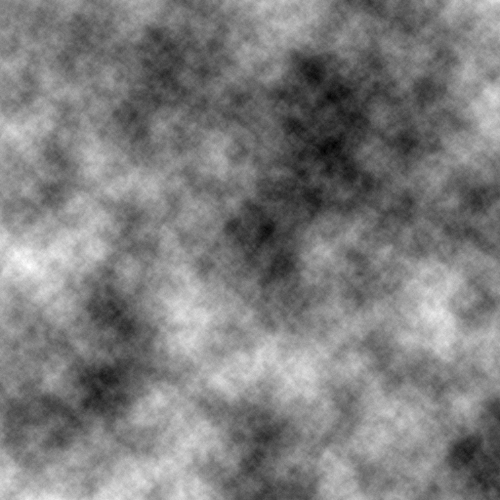
\includegraphics[width=0.9\linewidth]{images/FracBrownMotion.png}
  \caption{Height map generated with Fractional Brownian Motion}
  \label{fig:sub2}
\end{subfigure}
\caption[Noise comparison]{\textit{Comparison of noise functions}}
\label{fig:R_kitchen_example}
\end{figure}

\subsubsection{Ground}
The ground is textured using a non-linear multi-texturing approach based on both altitude and terrain slope. Currently only three textures are used, one sandy, one grassy and one rocky. ... TODO: blah...\\
\\
FIGURE(comparison of texturing)
\\
FIGURE(comparison of texturing)
\\

\subsubsection{Green stuff}
In order for the world to be more interesting than just an island in the middle of the sea, it needs some additional objects aswell, thus plants are placed using two slightly different approaches.

First a base layer of smaller bushes are placed uniformly over the landmass, with a randomized orientation and scaling. Then a few points are designated as forest centers, around these trees are placed using a gaussian distribution, again the trees have some scale and rotation randomly selected.

Placing the objects is done by generating a coordinate, and checking it for suitability, for example nothing can be placed in the water, or to far up on a mountain/voulcano.

\begin{figure}[H]
  \centering
  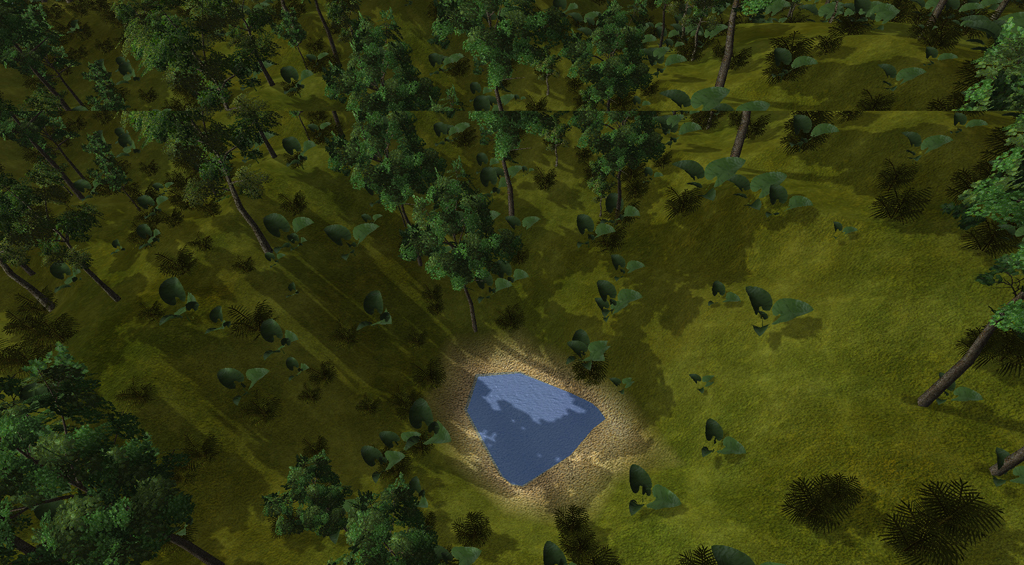
\includegraphics[width=0.9\linewidth]{images/content1.eps}
  \caption{A small water hole in the middle of the forest at the late afternoon.}
  \label{fig:water_hole}
\end{figure}%

\subsubsection{Volcano}
\begin{figure}[H]
  \centering
  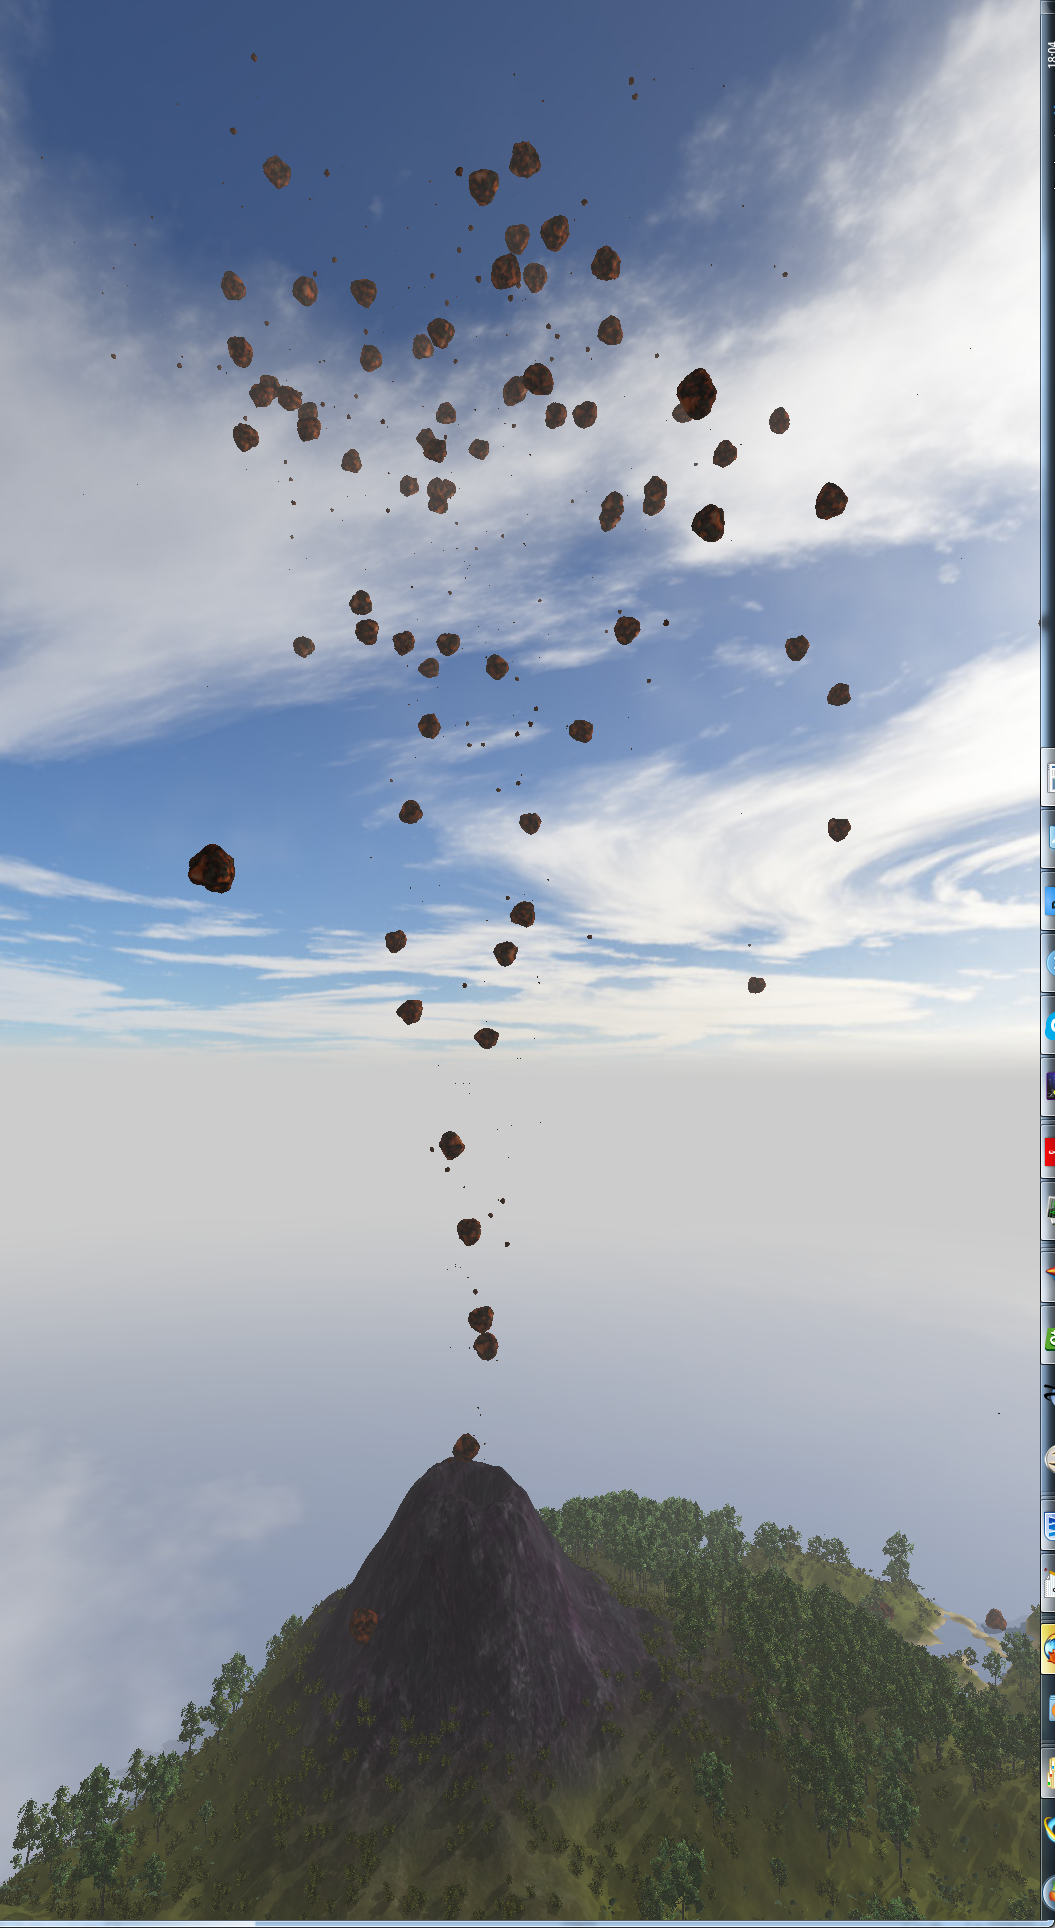
\includegraphics[width=0.8\linewidth]{images/volcano.png}
  \caption{A vulcano.}
  \label{fig:vulcano}
\end{figure}%
// TODO - Tigerwra\\
\\
The volcano is made up of the addition and the subtraction..\\
\\
When the fire balls enter the water and sink too deep, they are re-spawned in the volcano and sent out though the hole again.
\\
\\
The physics can be reversed in time, and balls returning to the volcano hole is then placed where they were when they disappeared, with all the physical properties reset to how they were at that time as well.
\\
\begin{figure}[H]
\begin{subfigure}{\textwidth}
  \centering
  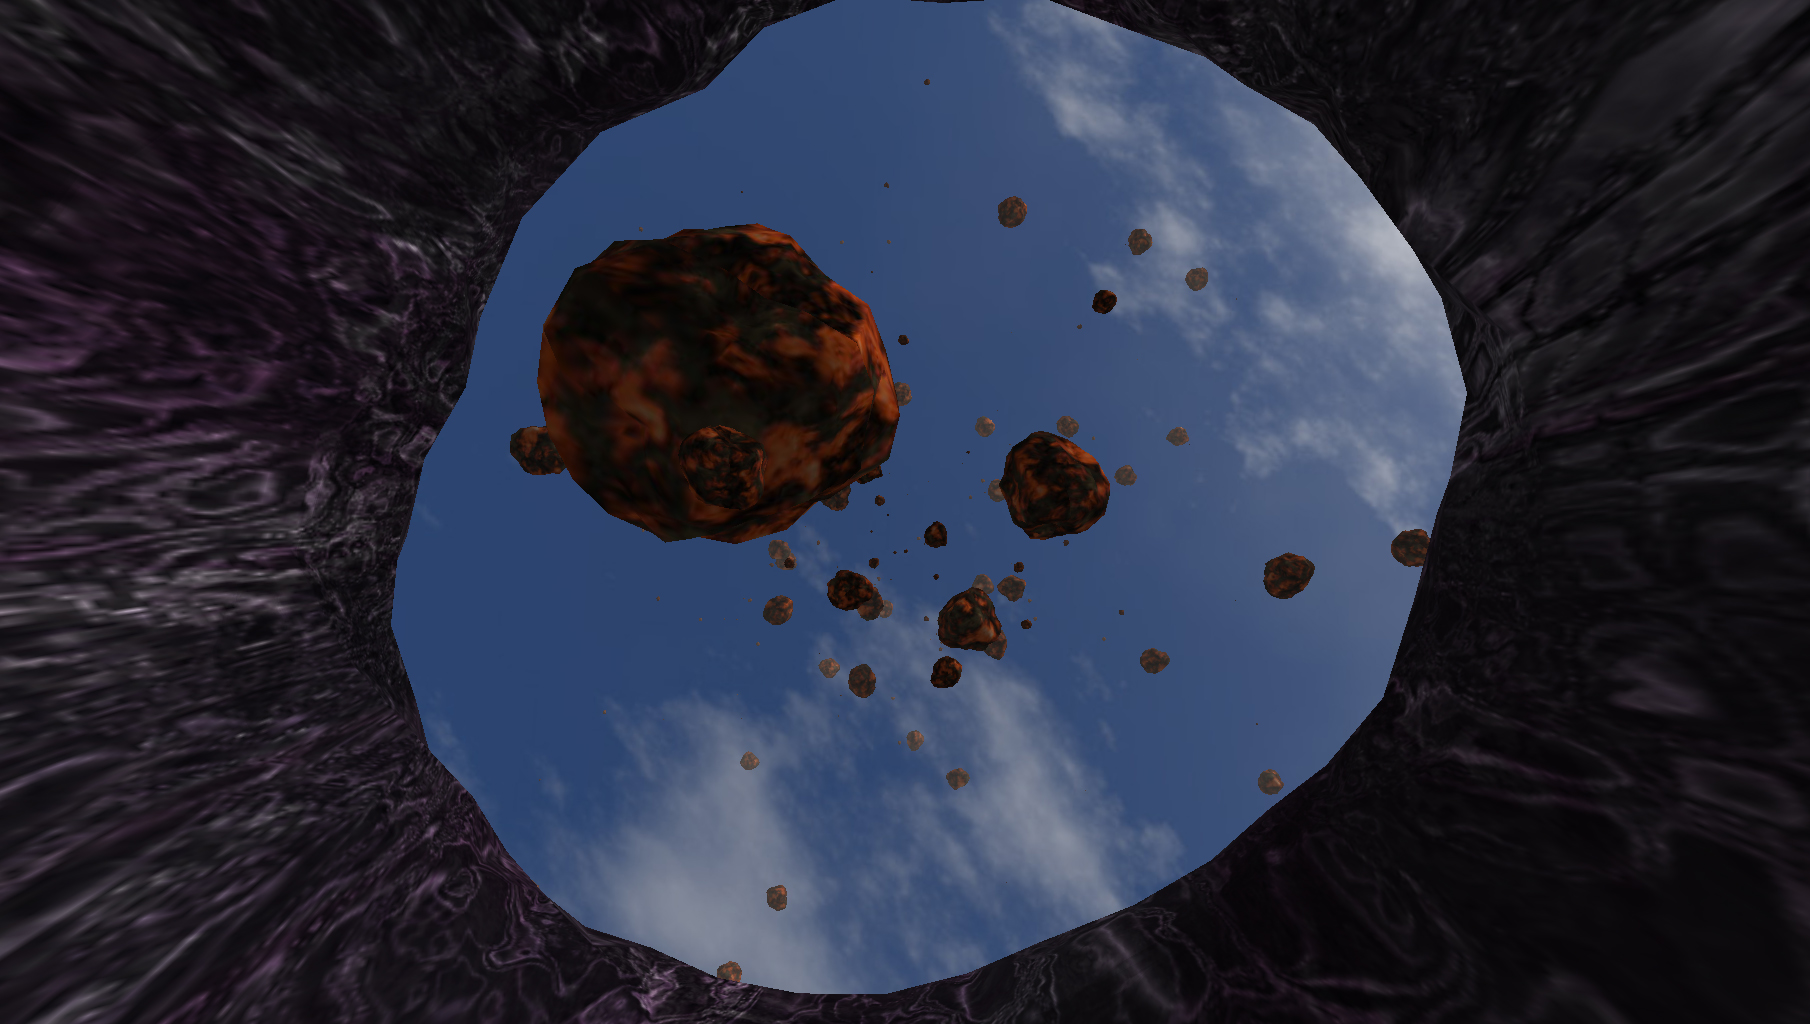
\includegraphics[width=0.9\linewidth]{images/Volcano1.eps}
  \caption{...}
  \label{fig:vulcano1}
\end{subfigure}%
\\
\begin{subfigure}{\textwidth}
  \centering
  \includegraphics[width=0.9\linewidth]{images/Volcano2.eps}
  \caption{...}
  \label{fig:vulcano2}
\end{subfigure}
\caption[Noise comparison]{\textit{Comparison of noise functions}}
\label{fig:vulcano3}
\end{figure}





\subsection{Visual Effects}
Boom hacka lacka

\subsubsection{Shadows}
Shadows are one those things that can make a scene really come to life. It will help the viewer to understand the structure of the terrain and location of objects. There are many techniques in which shadows can be achieved with different pros and cons. We have chosen to use shadow mapping since it offers real-time shadows for arbitrary shapes in a theoretically straight forward way. 

The quality of these can be increased arbitrarily, but the computational complexity is increased equivalently, which is what limits this method. 

More specifically our implementation utilizes \textit{Light-Space Shadow Mapping} which can be summarized in the following steps:

\begin{itemize}
\item Place the camera in the light source and adjust the camera frustum to cover the part of the scene that will be visible in the final render.
\item Render the scene with as simple shaders as possible and store the depth buffer. This is the shadow map.
\item Place the camera in its final-render location.
\item For each vertex:
\begin{itemize}
\item Transform into light-space coordinates.
\item Compare the distance from the light source with the corresponding value in the shadow map.
\item If the vertex is further away than the shadow map suggests, it will be shadowed. 
\end{itemize}
\end{itemize}

\begin{figure}[H]
\begin{subfigure}{.33\textwidth}
  \centering
  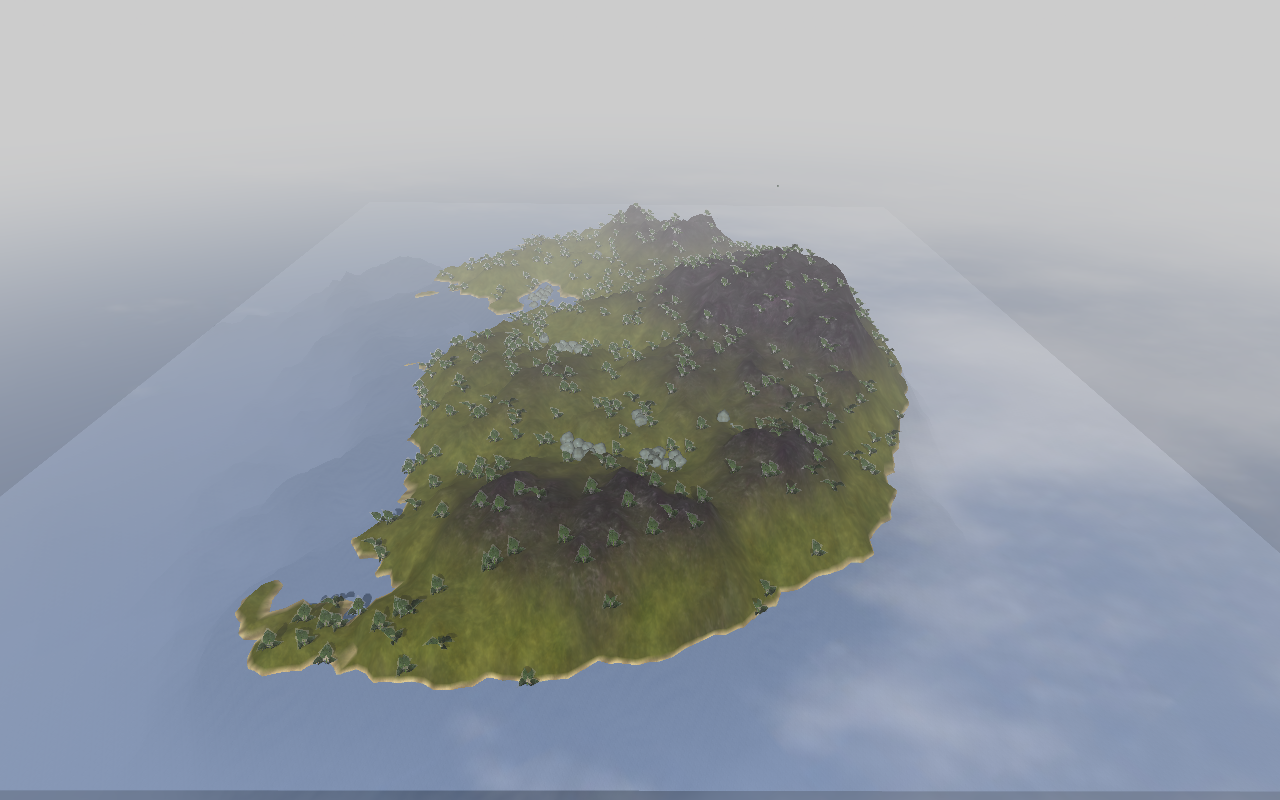
\includegraphics[width=0.9\linewidth]{images/SMOverViewLvl1.png}
  \caption{Shadow mapping level 1}
  \label{fig:SMOverViewLvl1}
\end{subfigure}%
\begin{subfigure}{.33\textwidth}
  \centering
  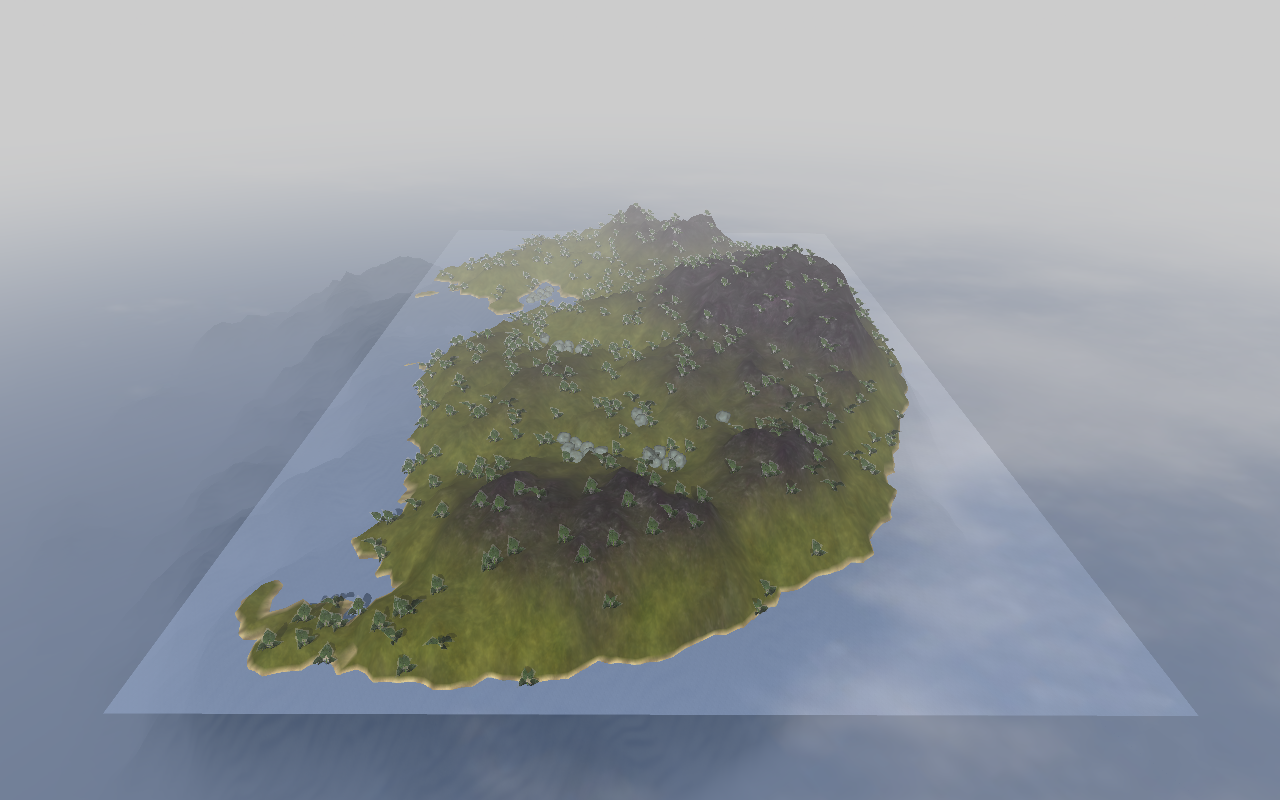
\includegraphics[width=0.9\linewidth]{images/SMOverViewLvl2.png}
  \caption{Shadow mapping level 2}
  \label{fig:SMOverViewLvl1}
\end{subfigure}
\begin{subfigure}{.33\textwidth}
  \centering
  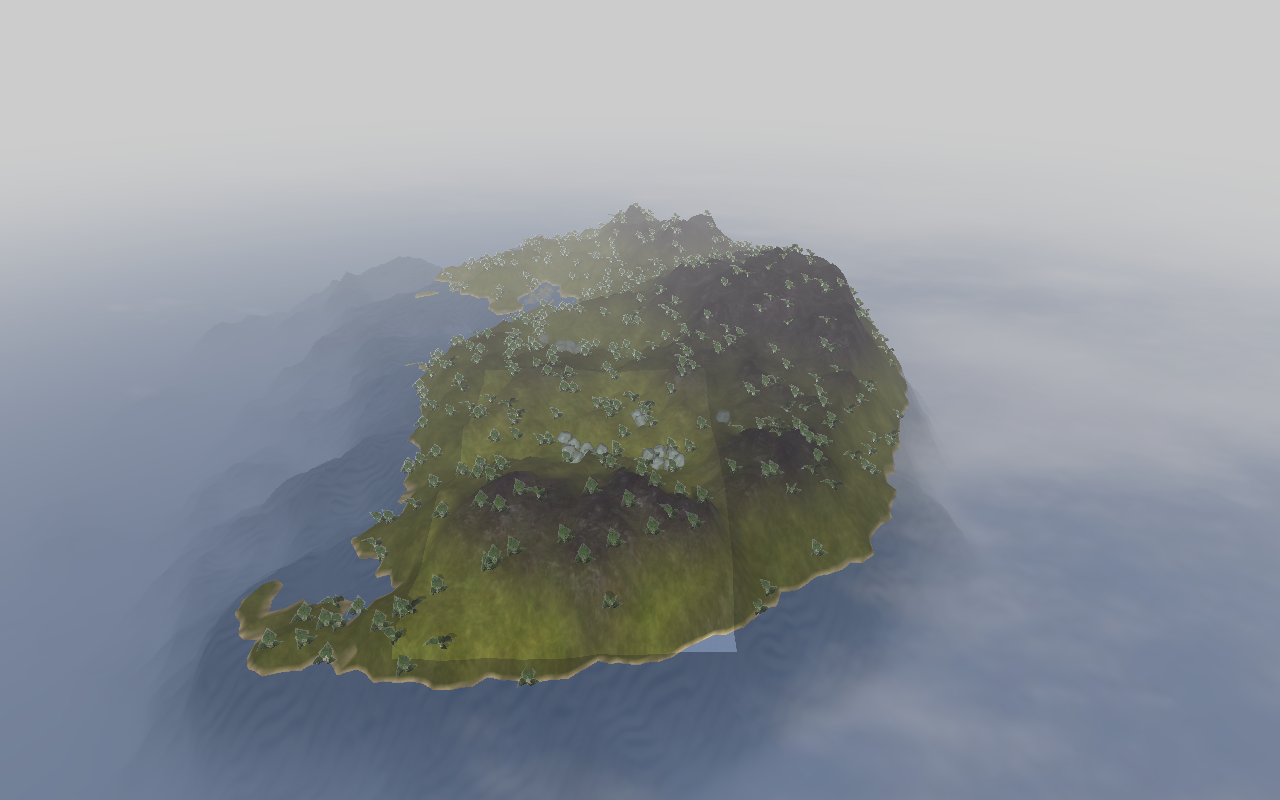
\includegraphics[width=0.9\linewidth]{images/SMOverViewLvl3.png}
  \caption{Shadow mapping level 3}
  \label{fig:SMOverViewLvl1}
\end{subfigure}
\caption[Noise comparison]{\textit{Overview of different shadow mapping levels}}
\label{fig:SMOverViewComparison}
\end{figure}

\begin{figure}[H]
\begin{subfigure}{.33\textwidth}
  \centering
  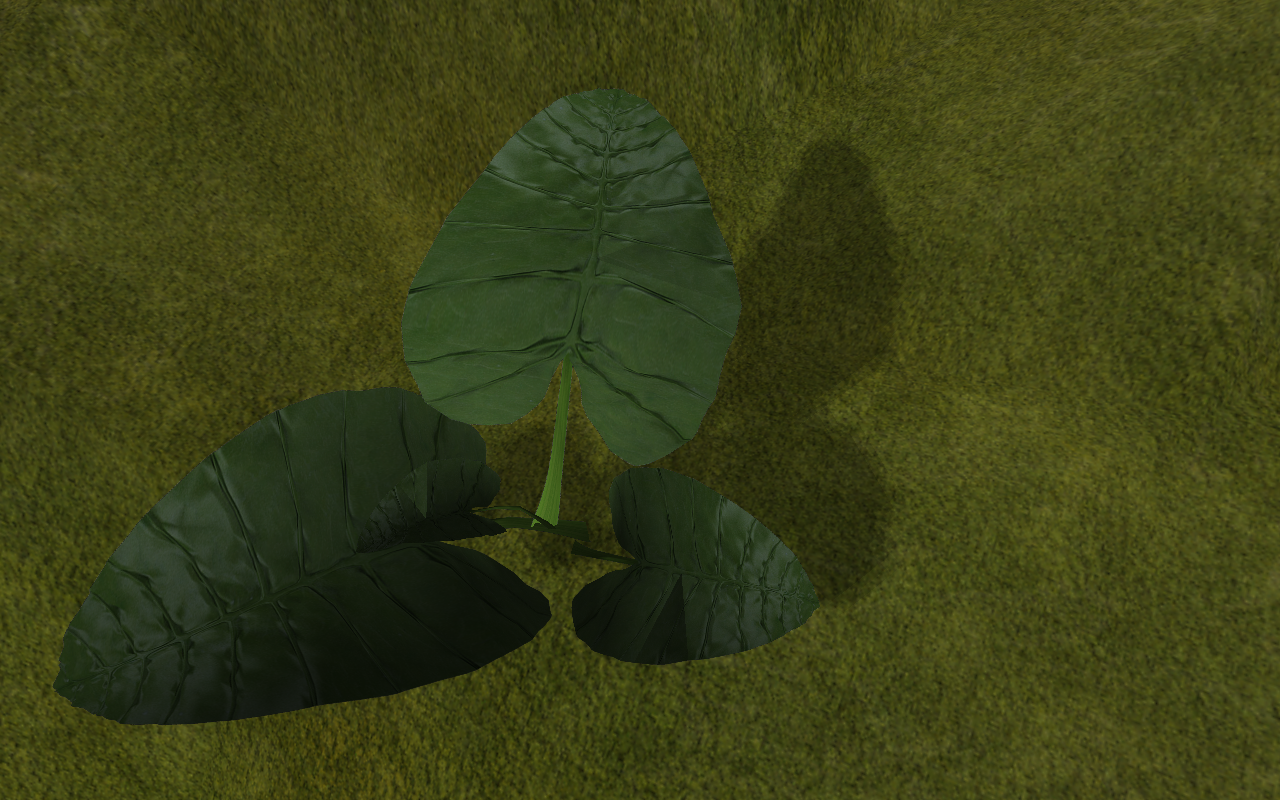
\includegraphics[width=0.9\linewidth]{images/SMCloseUpLvl1.png}
  \caption{Shadow mapping level 1}
  \label{fig:SMCloseUpLvl1}
\end{subfigure}%
\begin{subfigure}{.33\textwidth}
  \centering
  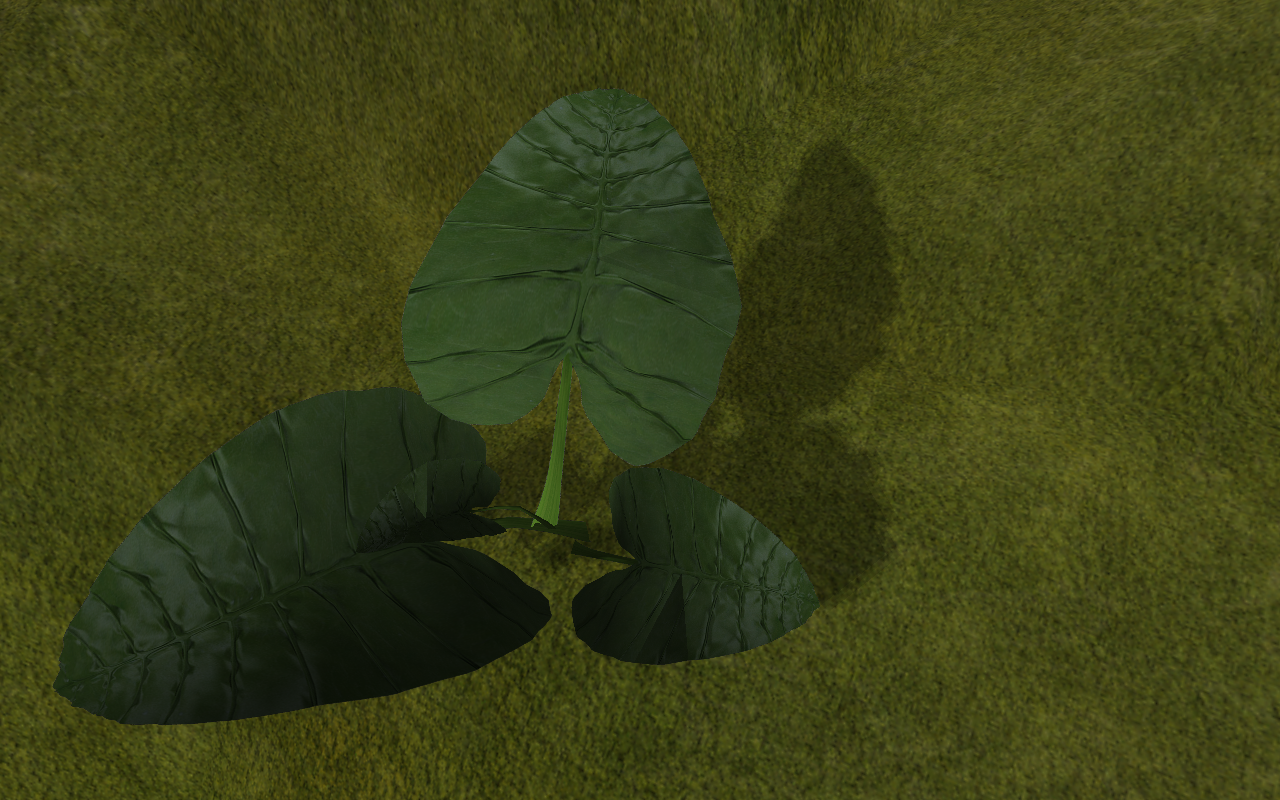
\includegraphics[width=0.9\linewidth]{images/SMCloseUpLvl2.png}
  \caption{Shadow mapping level 2}
  \label{fig:SMCloseUpLvl1}
\end{subfigure}
\begin{subfigure}{.33\textwidth}
  \centering
  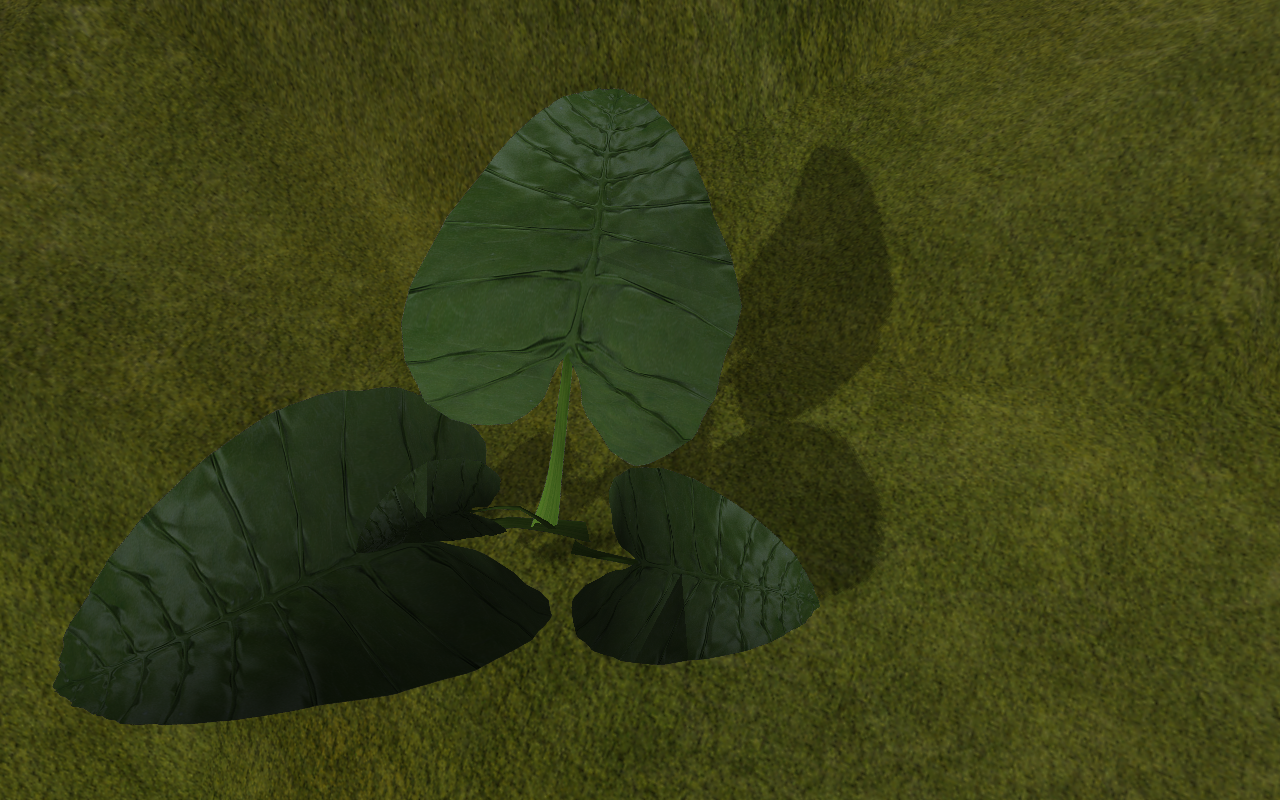
\includegraphics[width=0.9\linewidth]{images/SMCloseUpLvl3.png}
  \caption{Shadow mapping level 3}
  \label{fig:SMCloseUpLvl1}
\end{subfigure}
\caption[Noise comparison]{\textit{Close-up of different shadow mapping levels}}
\label{fig:SMCloseUpComparison}
\end{figure}

\begin{figure}[H]
\begin{subfigure}{.5\textwidth}
  \centering
  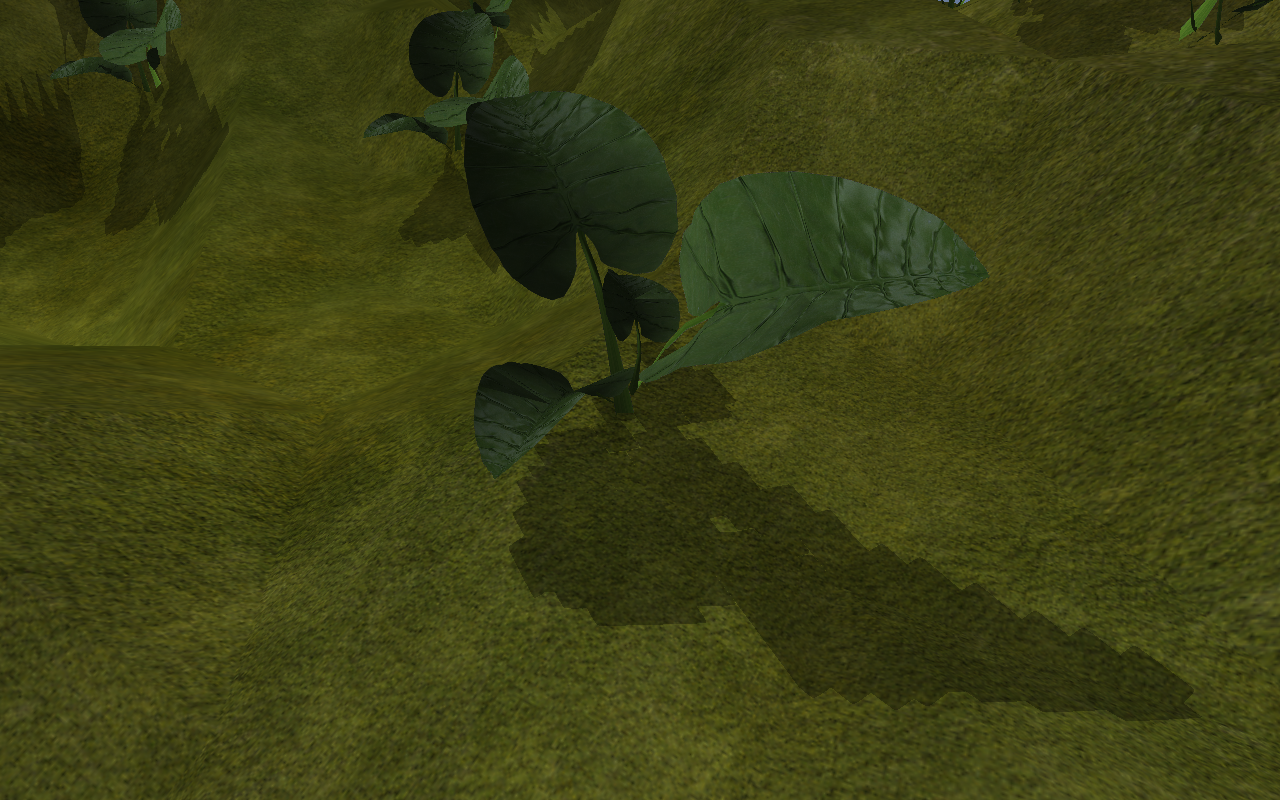
\includegraphics[width=0.9\linewidth]{images/PCFLvl1.png}
  \caption{Original skybox}
  \label{fig:PCFLvl1}
\end{subfigure}%
\begin{subfigure}{.5\textwidth}
  \centering
  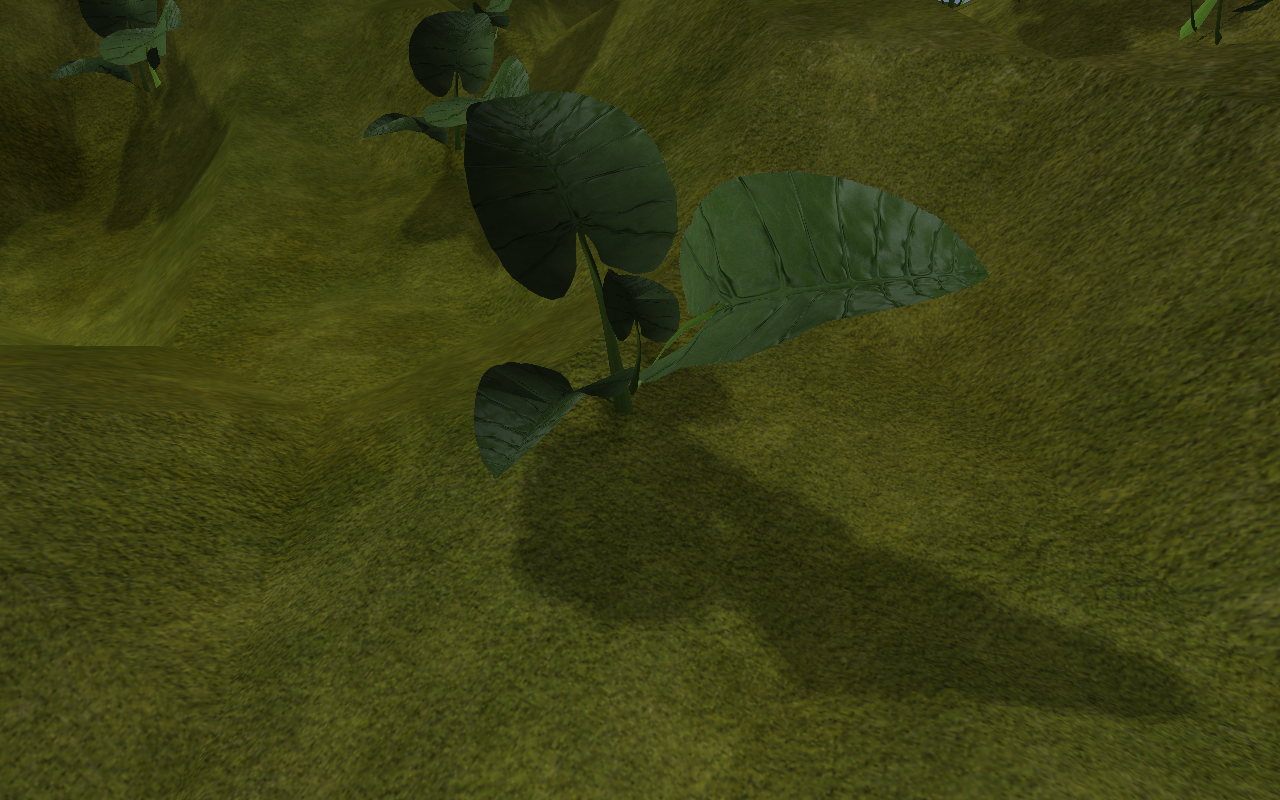
\includegraphics[width=0.9\linewidth]{images/PCFLvl5.png}
  \caption{Skybox modified to fade into fog}
  \label{fig:PCFLvl1}
\end{subfigure}
\caption[Noise comparison]{\textit{Comparison of shadow mapping with and without percentage-closer filtering}}
\label{fig:PCFComparison}
\end{figure}


\subsubsection{Fog}
The transition between different parts of the world can sometimes be very sharp in an unpleasant way. For instance, at the border between the sky and the ocean seen in figure \ref{fig:HorizonNoFog}. 

This can be remedied be adding some distance-fog to the ocean. If the color of the fog matches the color of the skybox at its horizon the transition will be seamless. Our skybox has been modify to fade into the color of the fog at its horizon, which can be seen in figure \ref{fig:SkyboxComparison} below. Notice that we have chosen to not let the skybox be affected by any fog. By doing so one can always see the sky when looking up, which is rather pleasant. 

\begin{figure}[H]
\begin{subfigure}{.5\textwidth}
  \centering
  \includegraphics[width=0.9\linewidth]{images/horizonNoFog.png}
  \caption{Horizon without fog}
  \label{fig:HorizonNoFog}
\end{subfigure}%
\begin{subfigure}{.5\textwidth}
  \centering
  \includegraphics[width=0.9\linewidth]{images/horizonFog.png}
  \caption{Horizon with fog}
  \label{fig:HorizonFog}
\end{subfigure}
\caption[Noise comparison]{\textit{Comparison of noise functions}}
\label{fig:HorizonFogComparison}
\end{figure}

\begin{figure}[H]
\begin{subfigure}{.5\textwidth}
  \centering
  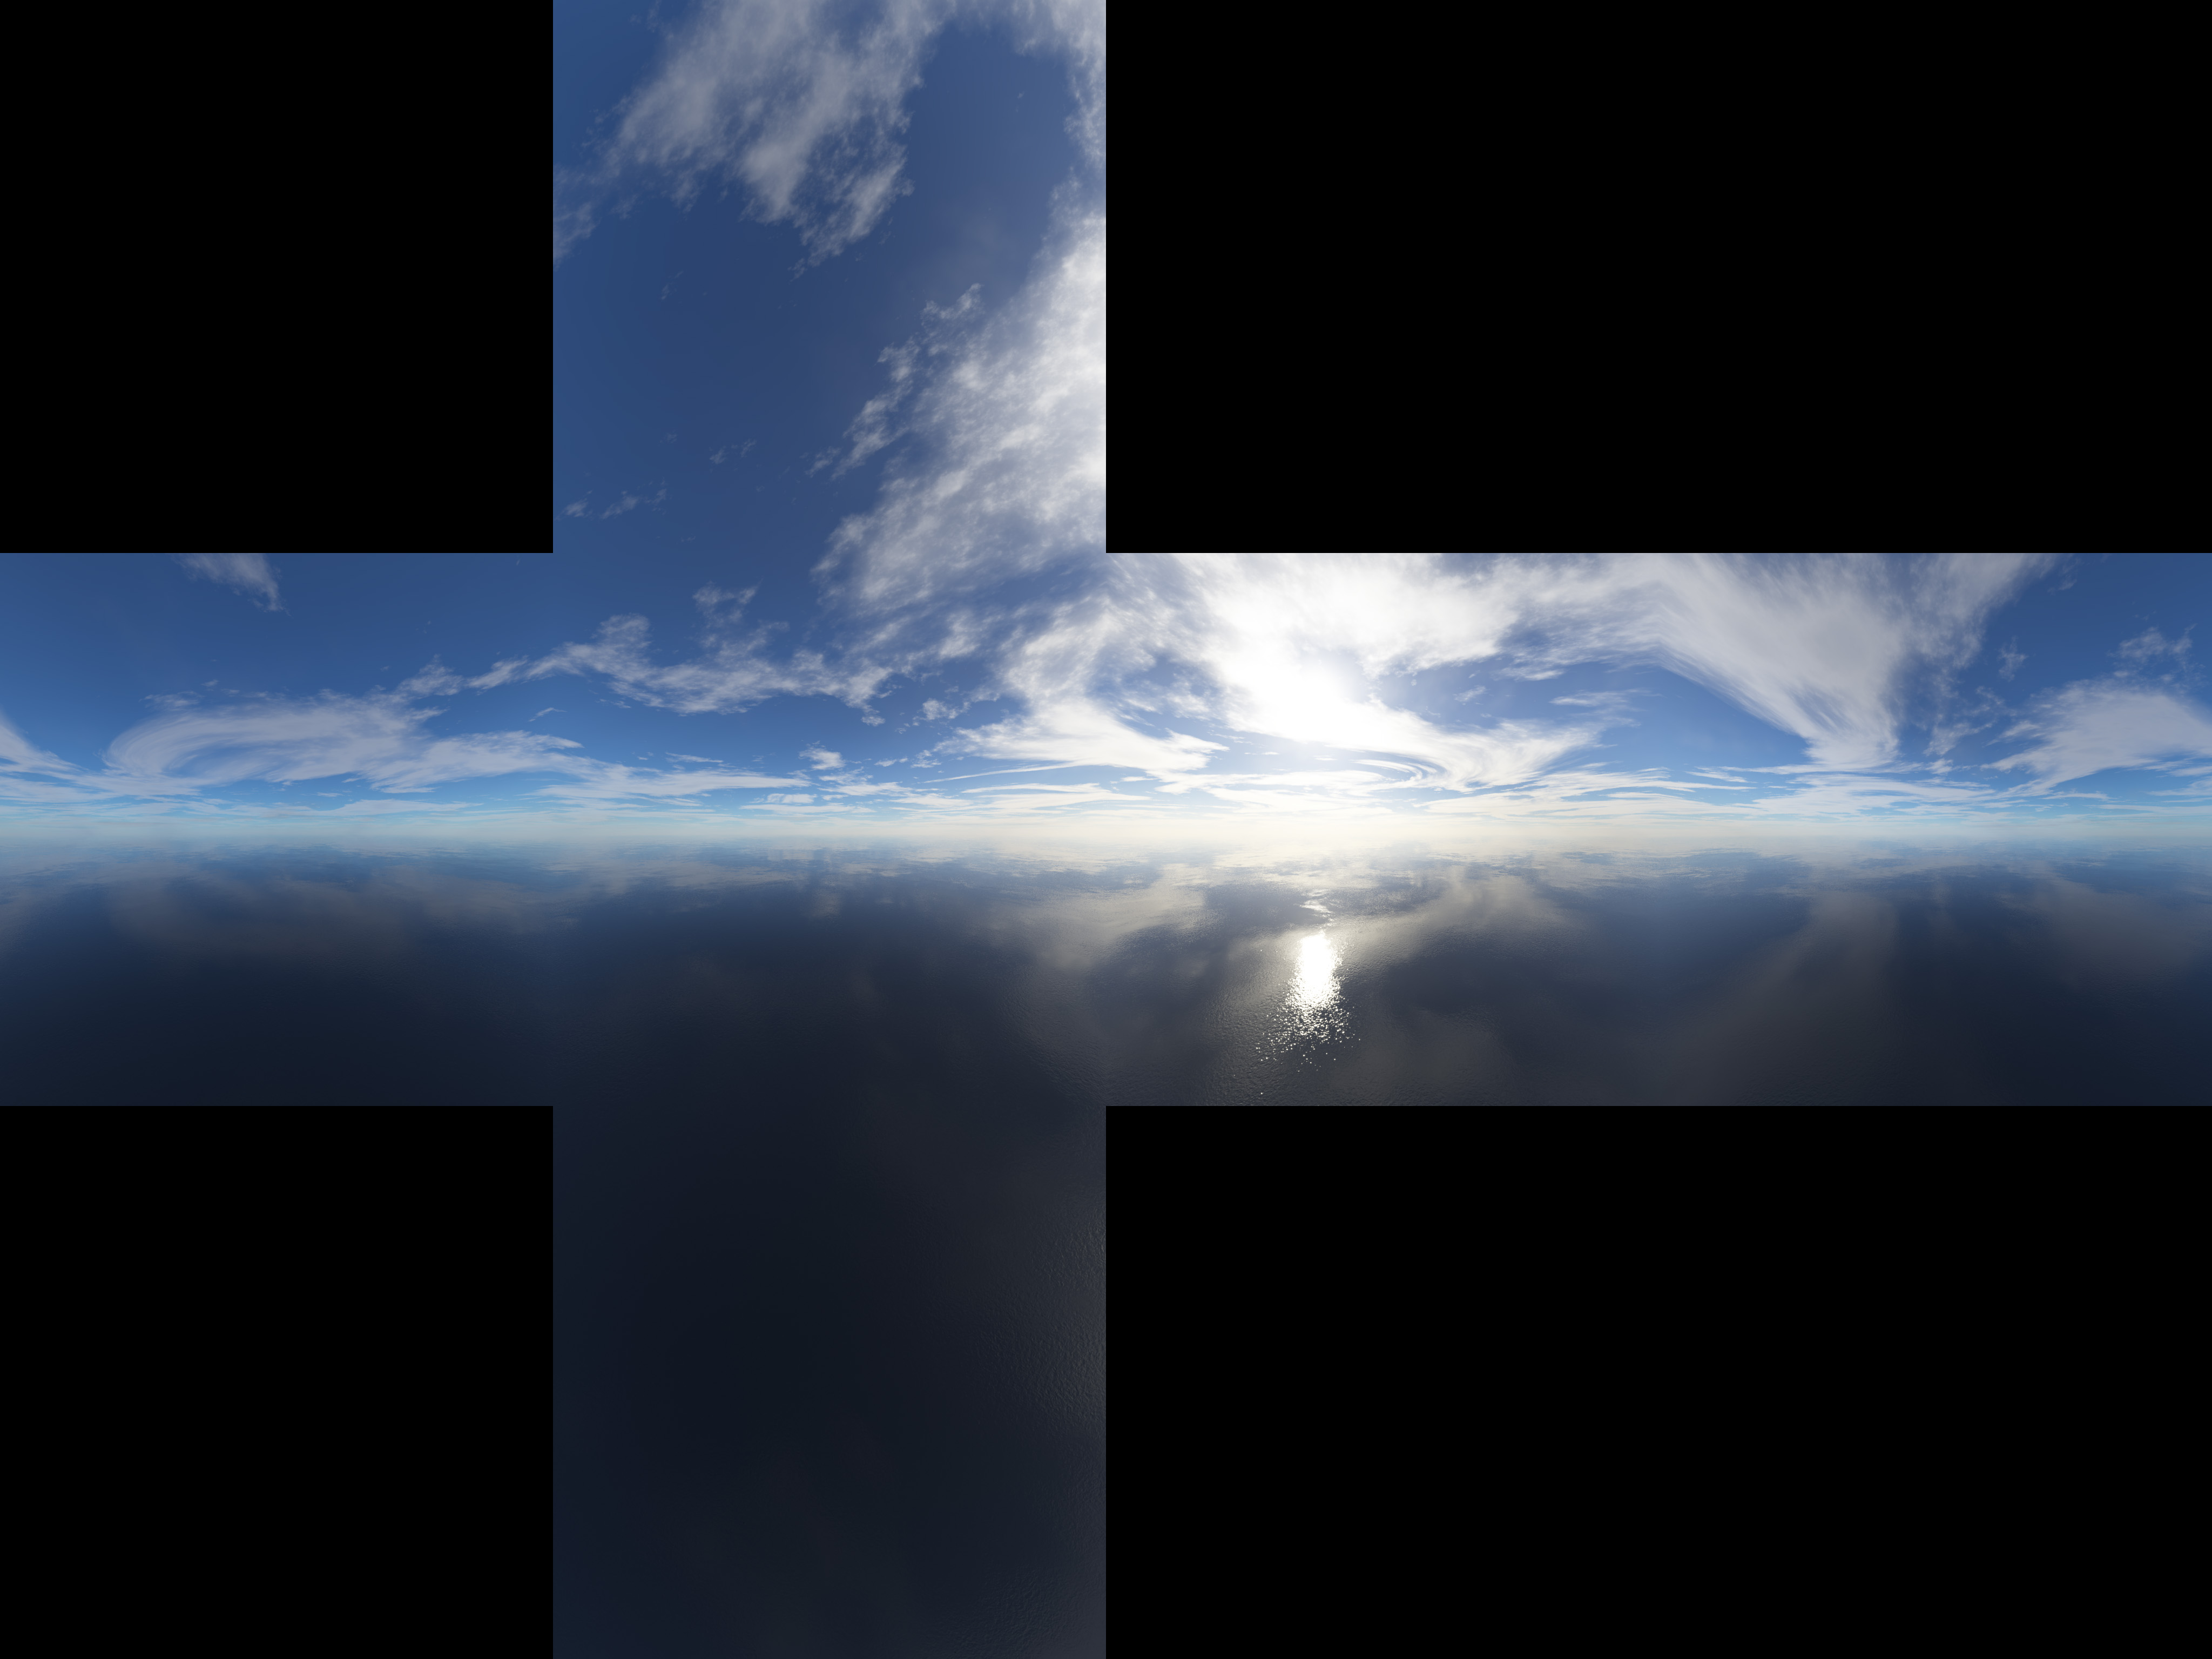
\includegraphics[width=0.9\linewidth]{images/skybox0.png}
  \caption{Original skybox}
  \label{fig:skybox0}
\end{subfigure}%
\begin{subfigure}{.5\textwidth}
  \centering
  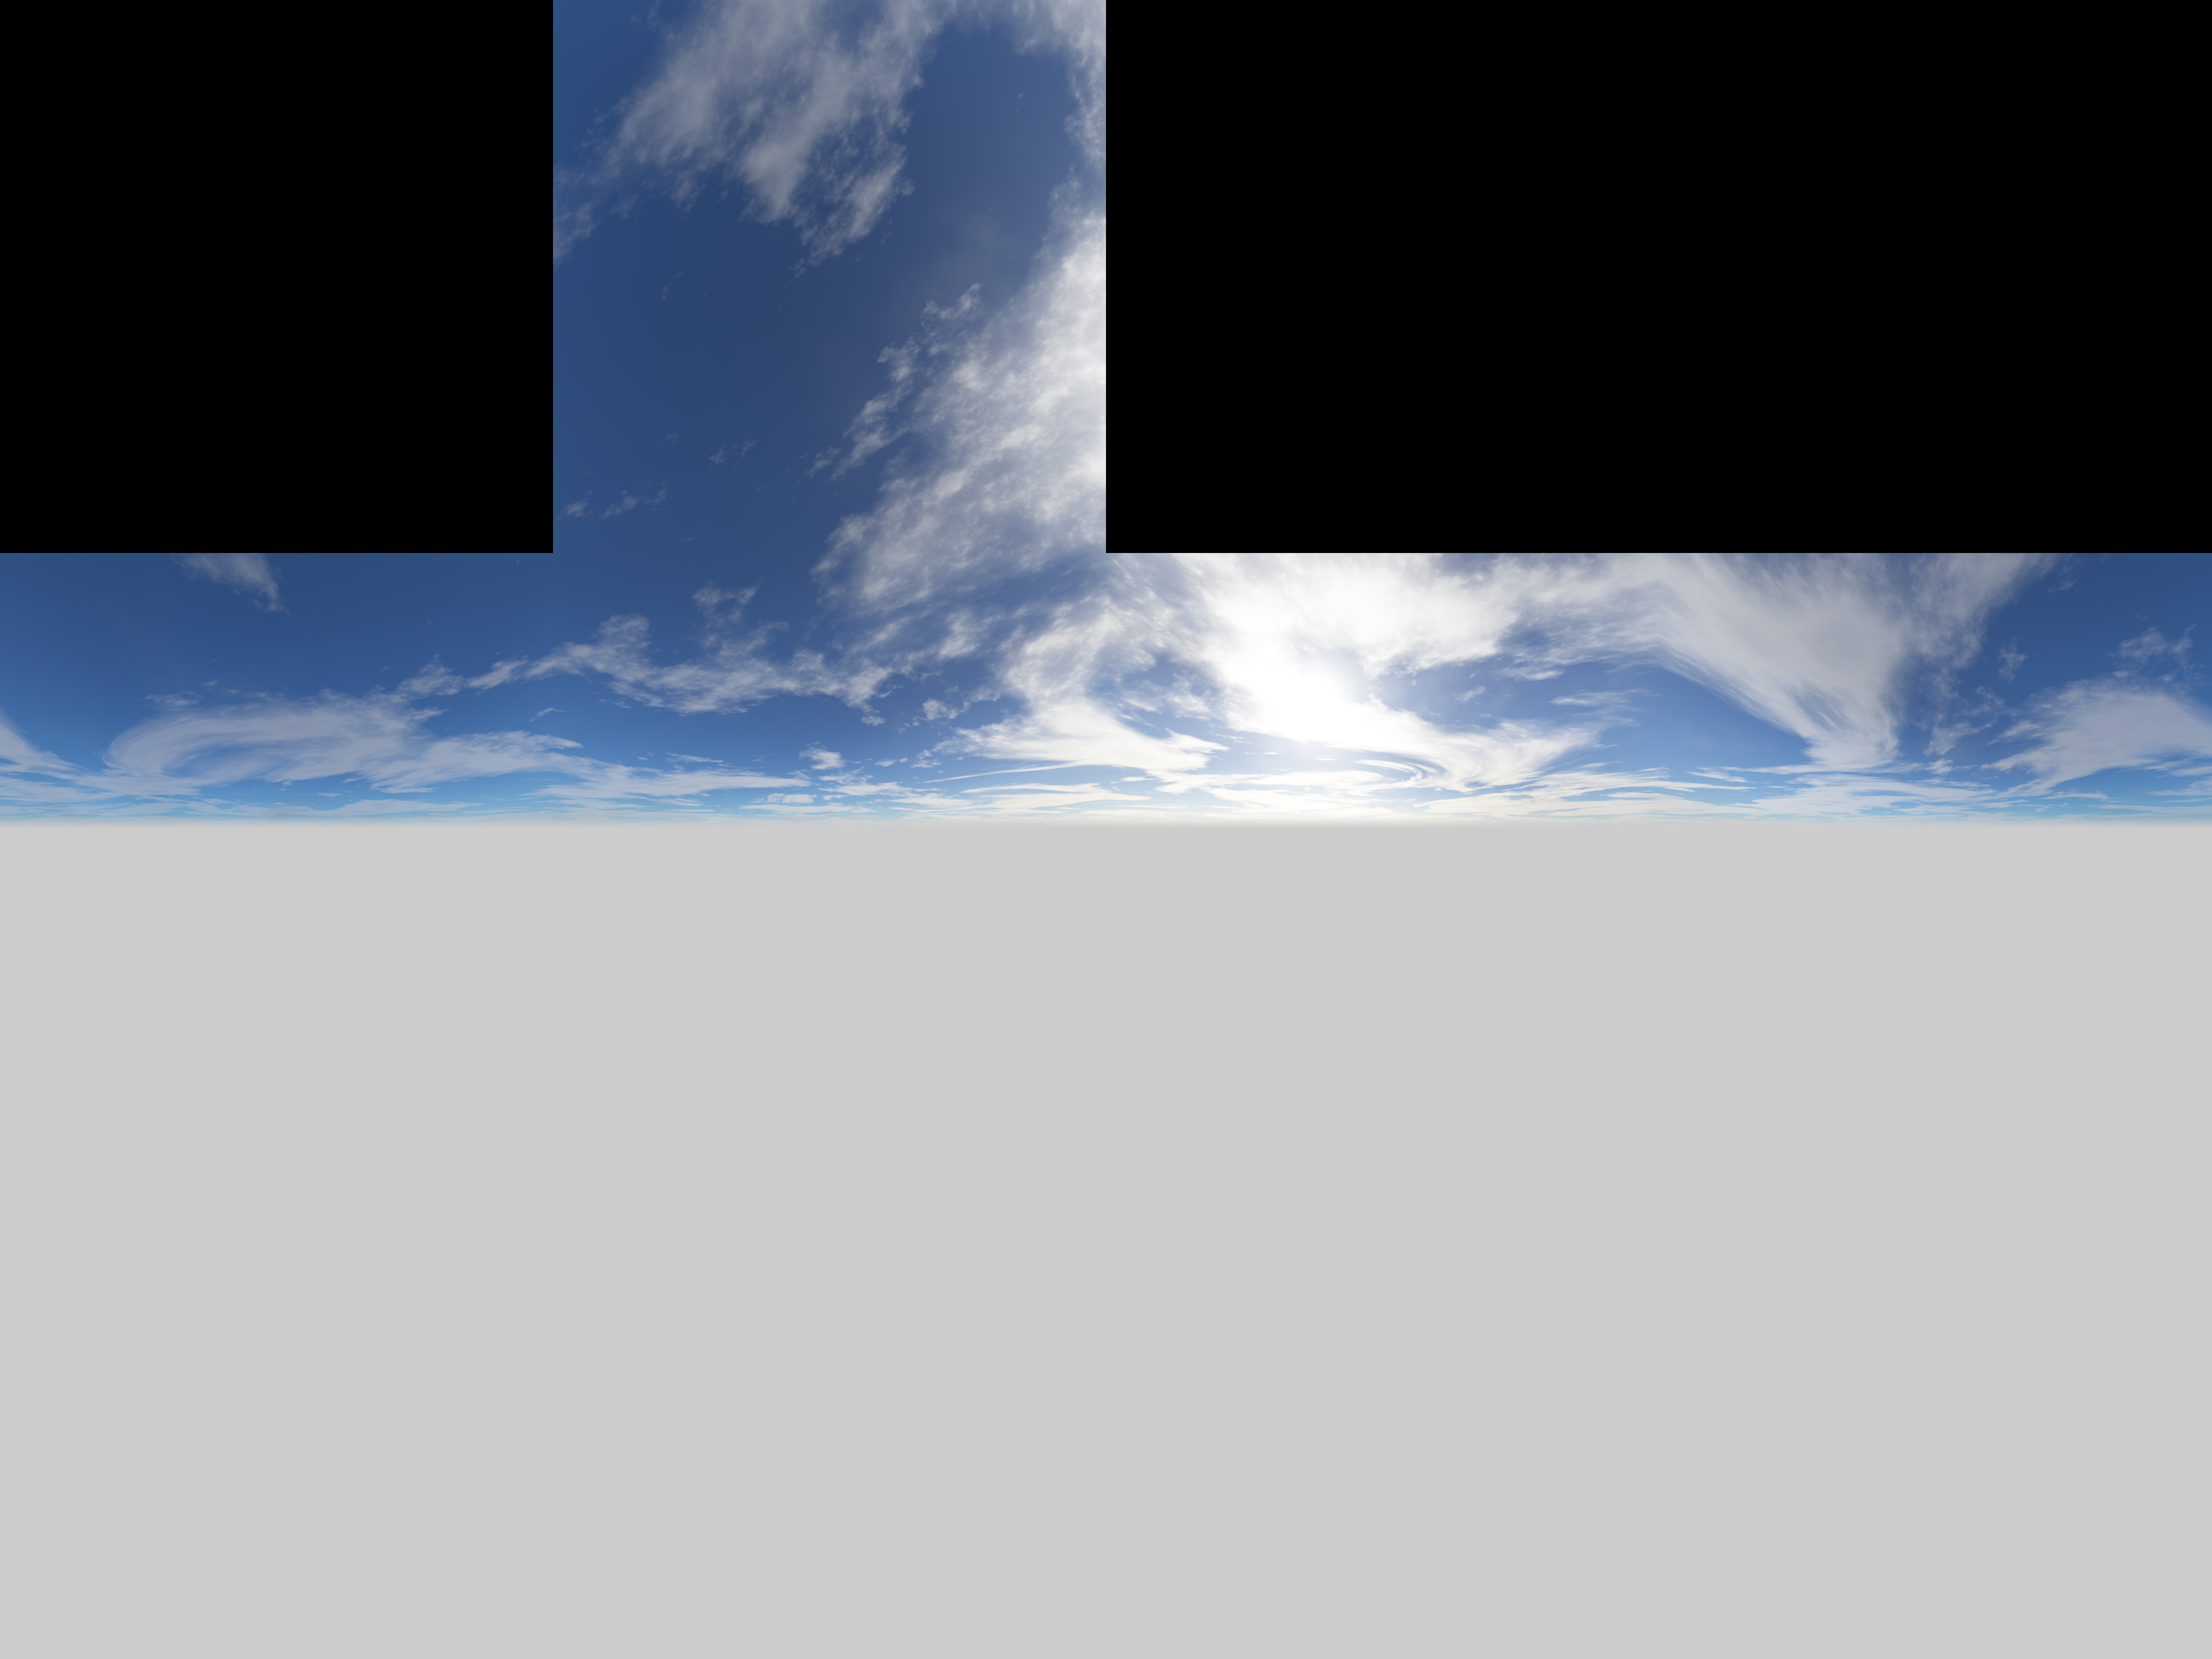
\includegraphics[width=0.9\linewidth]{images/skybox1.png}
  \caption{Skybox modified to fade into fog}
  \label{fig:skybox1}
\end{subfigure}
\caption[Noise comparison]{\textit{Comparison of skyboxes}}
\label{fig:SkyboxComparison}
\end{figure}

The distance-fog is also good for constraining the rendering size of the current scene. By adjusting the distance at which the fog appears one can adjust how much that is needed to be rendered of the scene. This enables an arbitrarily large world to be present without killing your computer since only the visible part of the world inside the fog-limit needs to be rendered. 

\subsubsection{Normal Mapping}
Normal mapping is a technique for adding fine details to an object without adding more vertices, which saves a lot of geometry computations. A normal map is generally an image where the RGB-channels represent x,y and z coordinates for a normal vector. This texture is used in the fragment shader when computing the shading for the current fragment. Before calculating the shading the normal vector is rotated to match the object on which it is to be mapped. Notice that the normal vector is not translated since we want it to remain as an normalized direction and nothing more. An example of a normal map can be seen in figure //TODO below.

// FIGURE









\newpage
\section{Artificial Intelligence}
\label{sec:AI}
Ai ai ai ai ai ai ai ai.


\newpage
\section{Conclusions}
\label{sec:conclusions}
Awesome




















%
% Bibliography
%

% Force a blank page so the bibliography starts on a new page.
% Comment out if not necessary
%\newpage
\thispagestyle{fancy}
\mbox{}
\begin{thebibliography}{9}
\addcontentsline{toc}{section}{References} % Add an entry for this in the table of contents

\bibitem{FracBrownMotion}
	Mandelbrot, B. \& Van Ness, J. (1968) \\ 
	``\textit{Fractional Brownian Motions, Fractional Noises and Applications}'' \\
	SIAM Review, Vol. 10, No. 4, pp. 422-437
	
\bibitem{ShadowMapping}
	Williams, L. (1978) \\ 
	``\textit{Casting Curved Shadows on Curved Surfaces}'' \\
	Computer Graphics Lab, New York Institute of Technology, Old Westbury, New York 11568 
	
\bibitem{ImprovedShadowMapping}
	Microsoft, Dev Center (2013) \\ 
	``\textit{Common Techniques to Improve Shadow Depth Maps}'' \\
	\href{http://msdn.microsoft.com/en-us/library/windows/desktop/ee416324(v=vs.85).aspx}{http://msdn.microsoft.com/en-us/library/windows/desktop/ee416324(v=vs.85).aspx}
	
\bibitem{CascadeShadowMapping}
	Microsoft, Dev Center (2013) \\ 
	``\textit{Cascaded Shadow Maps}'' \\
	\href{http://msdn.microsoft.com/en-us/library/windows/desktop/ee416307(v=vs.85).aspx}{http://msdn.microsoft.com/en-us/library/windows/desktop/ee416307(v=vs.85).aspx}

	
\bibitem{citekey}
\bibitem{citekey}

\bibitem{Gardel}
	Gardel, A., Bravo, I., Jimenez, P., Lazaro, J.L. \& Torquemada, A.\\
	``\textit{Statistical Background Models with Shadow Detection for Video Based Tracking},''\\ Intelligent Signal Processing, 2007. WISP 2007. IEEE International Symposium on?? Page: 1-6.
	
\bibitem{Zivkovic}
	Zivkovic, Z. \& Heijden, F.\\
	``\textit{Efficient Adaptive Density Estimation per Image Pixel for the Task of Background Subtraction},''\\
	Pattern recognition letters, Vol. 27, No. 7. (2006), pp. 773-780.

\bibitem{MOTA}
	Bernardin, K. \& Stiefelhagen, R (2008)\\
	``\textit{Evaluating Multiple Object Tracking Performance: The CLEAR MOT Metrics},''\\
	Interactive Systems Lab, Institut für Theoretische Informatik,\\
	Universität Karlsruhe, 76131 Karlsruhe, Germany
	
\bibitem{CAVIAR}
	``\textit{CAVIAR: Context Aware Vision using Image-based Active Recognition},''\\
	EC Funded CAVIAR project/IST 2001 37540\\
	http://homepages.inf.ed.ac.uk/rbf/CAVIAR/
	
\bibitem{StereoBM}
	Hirschmüller, H (2008)\\
	``\textit{Stereo Processing by Semiglobal Matching and Mutual Information},''\\
	IEEE Transactions on Pattern Analysis and Machine Intelligence, Volume 30(2)
	pp. 328-341.
	
\bibitem{OpenCV}
	OpenCV \textit{Open source computer vision}\\
	http://docs.opencv.org/\\
	Accessed on 2013-12-13\\
	

%\bibitem{somePaper}
%	Q. Lastname,
%	``Some article title,''
%	\emph{Some scientific journal},
%	vol.~1337, no.~1337,
%	pp.~666--1337,
%	month.~1337.

\end{thebibliography}



\end{document}
